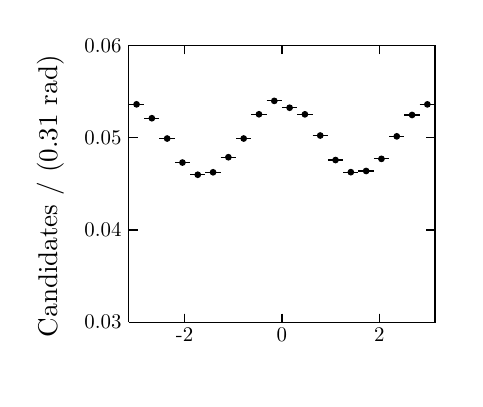
\begin{tikzpicture}
\pgfdeclareplotmark{cross} {
\pgfpathmoveto{\pgfpoint{-0.3\pgfplotmarksize}{\pgfplotmarksize}}
\pgfpathlineto{\pgfpoint{+0.3\pgfplotmarksize}{\pgfplotmarksize}}
\pgfpathlineto{\pgfpoint{+0.3\pgfplotmarksize}{0.3\pgfplotmarksize}}
\pgfpathlineto{\pgfpoint{+1\pgfplotmarksize}{0.3\pgfplotmarksize}}
\pgfpathlineto{\pgfpoint{+1\pgfplotmarksize}{-0.3\pgfplotmarksize}}
\pgfpathlineto{\pgfpoint{+0.3\pgfplotmarksize}{-0.3\pgfplotmarksize}}
\pgfpathlineto{\pgfpoint{+0.3\pgfplotmarksize}{-1.\pgfplotmarksize}}
\pgfpathlineto{\pgfpoint{-0.3\pgfplotmarksize}{-1.\pgfplotmarksize}}
\pgfpathlineto{\pgfpoint{-0.3\pgfplotmarksize}{-0.3\pgfplotmarksize}}
\pgfpathlineto{\pgfpoint{-1.\pgfplotmarksize}{-0.3\pgfplotmarksize}}
\pgfpathlineto{\pgfpoint{-1.\pgfplotmarksize}{0.3\pgfplotmarksize}}
\pgfpathlineto{\pgfpoint{-0.3\pgfplotmarksize}{0.3\pgfplotmarksize}}
\pgfpathclose
\pgfusepathqstroke
}
\pgfdeclareplotmark{cross*} {
\pgfpathmoveto{\pgfpoint{-0.3\pgfplotmarksize}{\pgfplotmarksize}}
\pgfpathlineto{\pgfpoint{+0.3\pgfplotmarksize}{\pgfplotmarksize}}
\pgfpathlineto{\pgfpoint{+0.3\pgfplotmarksize}{0.3\pgfplotmarksize}}
\pgfpathlineto{\pgfpoint{+1\pgfplotmarksize}{0.3\pgfplotmarksize}}
\pgfpathlineto{\pgfpoint{+1\pgfplotmarksize}{-0.3\pgfplotmarksize}}
\pgfpathlineto{\pgfpoint{+0.3\pgfplotmarksize}{-0.3\pgfplotmarksize}}
\pgfpathlineto{\pgfpoint{+0.3\pgfplotmarksize}{-1.\pgfplotmarksize}}
\pgfpathlineto{\pgfpoint{-0.3\pgfplotmarksize}{-1.\pgfplotmarksize}}
\pgfpathlineto{\pgfpoint{-0.3\pgfplotmarksize}{-0.3\pgfplotmarksize}}
\pgfpathlineto{\pgfpoint{-1.\pgfplotmarksize}{-0.3\pgfplotmarksize}}
\pgfpathlineto{\pgfpoint{-1.\pgfplotmarksize}{0.3\pgfplotmarksize}}
\pgfpathlineto{\pgfpoint{-0.3\pgfplotmarksize}{0.3\pgfplotmarksize}}
\pgfpathclose
\pgfusepathqfillstroke
}
\pgfdeclareplotmark{newstar} {
\pgfpathmoveto{\pgfqpoint{0pt}{\pgfplotmarksize}}
\pgfpathlineto{\pgfqpointpolar{44}{0.5\pgfplotmarksize}}
\pgfpathlineto{\pgfqpointpolar{18}{\pgfplotmarksize}}
\pgfpathlineto{\pgfqpointpolar{-20}{0.5\pgfplotmarksize}}
\pgfpathlineto{\pgfqpointpolar{-54}{\pgfplotmarksize}}
\pgfpathlineto{\pgfqpointpolar{-90}{0.5\pgfplotmarksize}}
\pgfpathlineto{\pgfqpointpolar{234}{\pgfplotmarksize}}
\pgfpathlineto{\pgfqpointpolar{198}{0.5\pgfplotmarksize}}
\pgfpathlineto{\pgfqpointpolar{162}{\pgfplotmarksize}}
\pgfpathlineto{\pgfqpointpolar{134}{0.5\pgfplotmarksize}}
\pgfpathclose
\pgfusepathqstroke
}
\pgfdeclareplotmark{newstar*} {
\pgfpathmoveto{\pgfqpoint{0pt}{\pgfplotmarksize}}
\pgfpathlineto{\pgfqpointpolar{44}{0.5\pgfplotmarksize}}
\pgfpathlineto{\pgfqpointpolar{18}{\pgfplotmarksize}}
\pgfpathlineto{\pgfqpointpolar{-20}{0.5\pgfplotmarksize}}
\pgfpathlineto{\pgfqpointpolar{-54}{\pgfplotmarksize}}
\pgfpathlineto{\pgfqpointpolar{-90}{0.5\pgfplotmarksize}}
\pgfpathlineto{\pgfqpointpolar{234}{\pgfplotmarksize}}
\pgfpathlineto{\pgfqpointpolar{198}{0.5\pgfplotmarksize}}
\pgfpathlineto{\pgfqpointpolar{162}{\pgfplotmarksize}}
\pgfpathlineto{\pgfqpointpolar{134}{0.5\pgfplotmarksize}}
\pgfpathclose
\pgfusepathqfillstroke
}
\definecolor{c}{rgb}{1,1,1};
\draw [color=c, fill=c] (5.1,4.72095) rectangle (9.9,9.16419);
\draw [color=c, fill=c] (5.772,5.43186) rectangle (9.66,8.94203);
\definecolor{c}{rgb}{0,0,0};
\draw [c] (5.772,5.43186) -- (5.772,8.94203) -- (9.66,8.94203) -- (9.66,5.43186) -- (5.772,5.43186);
\draw [c,line width=0.4] (5.8692,8.17042) -- (5.8692,8.19752);
\draw [c,line width=0.4] (5.8692,8.19752) -- (5.8692,8.22462);
\draw [c,line width=0.4] (5.772,8.19752) -- (5.8692,8.19752);
\draw [c,line width=0.4] (5.8692,8.19752) -- (5.9664,8.19752);
\foreach \P in {(5.8692,8.19752)}{\draw[mark options={color=c,fill=c},mark size=1.201201pt,mark=*,mark size=1pt] plot coordinates {\P};}
\draw [c,line width=0.4] (6.0636,7.99448) -- (6.0636,8.02119);
\draw [c,line width=0.4] (6.0636,8.02119) -- (6.0636,8.04791);
\draw [c,line width=0.4] (5.9664,8.02119) -- (6.0636,8.02119);
\draw [c,line width=0.4] (6.0636,8.02119) -- (6.1608,8.02119);
\foreach \P in {(6.0636,8.02119)}{\draw[mark options={color=c,fill=c},mark size=1.201201pt,mark=*,mark size=1pt] plot coordinates {\P};}
\draw [c,line width=0.4] (6.258,7.73705) -- (6.258,7.7632);
\draw [c,line width=0.4] (6.258,7.7632) -- (6.258,7.78934);
\draw [c,line width=0.4] (6.1608,7.7632) -- (6.258,7.7632);
\draw [c,line width=0.4] (6.258,7.7632) -- (6.3552,7.7632);
\foreach \P in {(6.258,7.7632)}{\draw[mark options={color=c,fill=c},mark size=1.201201pt,mark=*,mark size=1pt] plot coordinates {\P};}
\draw [c,line width=0.4] (6.4524,7.43271) -- (6.4524,7.45816);
\draw [c,line width=0.4] (6.4524,7.45816) -- (6.4524,7.48362);
\draw [c,line width=0.4] (6.3552,7.45816) -- (6.4524,7.45816);
\draw [c,line width=0.4] (6.4524,7.45816) -- (6.5496,7.45816);
\foreach \P in {(6.4524,7.45816)}{\draw[mark options={color=c,fill=c},mark size=1.201201pt,mark=*,mark size=1pt] plot coordinates {\P};}
\draw [c,line width=0.4] (6.6468,7.27816) -- (6.6468,7.30325);
\draw [c,line width=0.4] (6.6468,7.30325) -- (6.6468,7.32834);
\draw [c,line width=0.4] (6.5496,7.30325) -- (6.6468,7.30325);
\draw [c,line width=0.4] (6.6468,7.30325) -- (6.744,7.30325);
\foreach \P in {(6.6468,7.30325)}{\draw[mark options={color=c,fill=c},mark size=1.201201pt,mark=*,mark size=1pt] plot coordinates {\P};}
\draw [c,line width=0.4] (6.8412,7.30944) -- (6.8412,7.33461);
\draw [c,line width=0.4] (6.8412,7.33461) -- (6.8412,7.35977);
\draw [c,line width=0.4] (6.744,7.33461) -- (6.8412,7.33461);
\draw [c,line width=0.4] (6.8412,7.33461) -- (6.9384,7.33461);
\foreach \P in {(6.8412,7.33461)}{\draw[mark options={color=c,fill=c},mark size=1.201201pt,mark=*,mark size=1pt] plot coordinates {\P};}
\draw [c,line width=0.4] (7.0356,7.50007) -- (7.0356,7.52568);
\draw [c,line width=0.4] (7.0356,7.52568) -- (7.0356,7.55128);
\draw [c,line width=0.4] (6.9384,7.52568) -- (7.0356,7.52568);
\draw [c,line width=0.4] (7.0356,7.52568) -- (7.1328,7.52568);
\foreach \P in {(7.0356,7.52568)}{\draw[mark options={color=c,fill=c},mark size=1.201201pt,mark=*,mark size=1pt] plot coordinates {\P};}
\draw [c,line width=0.4] (7.23,7.73729) -- (7.23,7.76343);
\draw [c,line width=0.4] (7.23,7.76343) -- (7.23,7.78958);
\draw [c,line width=0.4] (7.1328,7.76343) -- (7.23,7.76343);
\draw [c,line width=0.4] (7.23,7.76343) -- (7.3272,7.76343);
\foreach \P in {(7.23,7.76343)}{\draw[mark options={color=c,fill=c},mark size=1.201201pt,mark=*,mark size=1pt] plot coordinates {\P};}
\draw [c,line width=0.4] (7.4244,8.04468) -- (7.4244,8.07151);
\draw [c,line width=0.4] (7.4244,8.07151) -- (7.4244,8.09833);
\draw [c,line width=0.4] (7.3272,8.07151) -- (7.4244,8.07151);
\draw [c,line width=0.4] (7.4244,8.07151) -- (7.5216,8.07151);
\foreach \P in {(7.4244,8.07151)}{\draw[mark options={color=c,fill=c},mark size=1.201201pt,mark=*,mark size=1pt] plot coordinates {\P};}
\draw [c,line width=0.4] (7.6188,8.21421) -- (7.6188,8.2414);
\draw [c,line width=0.4] (7.6188,8.2414) -- (7.6188,8.26859);
\draw [c,line width=0.4] (7.5216,8.2414) -- (7.6188,8.2414);
\draw [c,line width=0.4] (7.6188,8.2414) -- (7.716,8.2414);
\foreach \P in {(7.6188,8.2414)}{\draw[mark options={color=c,fill=c},mark size=1.201201pt,mark=*,mark size=1pt] plot coordinates {\P};}
\draw [c,line width=0.4] (7.8132,8.12746) -- (7.8132,8.15446);
\draw [c,line width=0.4] (7.8132,8.15446) -- (7.8132,8.18147);
\draw [c,line width=0.4] (7.716,8.15446) -- (7.8132,8.15446);
\draw [c,line width=0.4] (7.8132,8.15446) -- (7.9104,8.15446);
\foreach \P in {(7.8132,8.15446)}{\draw[mark options={color=c,fill=c},mark size=1.201201pt,mark=*,mark size=1pt] plot coordinates {\P};}
\draw [c,line width=0.4] (8.0076,8.04375) -- (8.0076,8.07057);
\draw [c,line width=0.4] (8.0076,8.07057) -- (8.0076,8.09739);
\draw [c,line width=0.4] (7.9104,8.07057) -- (8.0076,8.07057);
\draw [c,line width=0.4] (8.0076,8.07057) -- (8.1048,8.07057);
\foreach \P in {(8.0076,8.07057)}{\draw[mark options={color=c,fill=c},mark size=1.201201pt,mark=*,mark size=1pt] plot coordinates {\P};}
\draw [c,line width=0.4] (8.202,7.77535) -- (8.202,7.80158);
\draw [c,line width=0.4] (8.202,7.80158) -- (8.202,7.8278);
\draw [c,line width=0.4] (8.1048,7.80158) -- (8.202,7.80158);
\draw [c,line width=0.4] (8.202,7.80158) -- (8.2992,7.80158);
\foreach \P in {(8.202,7.80158)}{\draw[mark options={color=c,fill=c},mark size=1.201201pt,mark=*,mark size=1pt] plot coordinates {\P};}
\draw [c,line width=0.4] (8.3964,7.46447) -- (8.3964,7.48999);
\draw [c,line width=0.4] (8.3964,7.48999) -- (8.3964,7.51551);
\draw [c,line width=0.4] (8.2992,7.48999) -- (8.3964,7.48999);
\draw [c,line width=0.4] (8.3964,7.48999) -- (8.4936,7.48999);
\foreach \P in {(8.3964,7.48999)}{\draw[mark options={color=c,fill=c},mark size=1.201201pt,mark=*,mark size=1pt] plot coordinates {\P};}
\draw [c,line width=0.4] (8.5908,7.31096) -- (8.5908,7.33613);
\draw [c,line width=0.4] (8.5908,7.33613) -- (8.5908,7.3613);
\draw [c,line width=0.4] (8.4936,7.33613) -- (8.5908,7.33613);
\draw [c,line width=0.4] (8.5908,7.33613) -- (8.688,7.33613);
\foreach \P in {(8.5908,7.33613)}{\draw[mark options={color=c,fill=c},mark size=1.201201pt,mark=*,mark size=1pt] plot coordinates {\P};}
\draw [c,line width=0.4] (8.7852,7.32602) -- (8.7852,7.35122);
\draw [c,line width=0.4] (8.7852,7.35122) -- (8.7852,7.37643);
\draw [c,line width=0.4] (8.688,7.35122) -- (8.7852,7.35122);
\draw [c,line width=0.4] (8.7852,7.35122) -- (8.8824,7.35122);
\foreach \P in {(8.7852,7.35122)}{\draw[mark options={color=c,fill=c},mark size=1.201201pt,mark=*,mark size=1pt] plot coordinates {\P};}
\draw [c,line width=0.4] (8.9796,7.47952) -- (8.9796,7.50508);
\draw [c,line width=0.4] (8.9796,7.50508) -- (8.9796,7.53064);
\draw [c,line width=0.4] (8.8824,7.50508) -- (8.9796,7.50508);
\draw [c,line width=0.4] (8.9796,7.50508) -- (9.0768,7.50508);
\foreach \P in {(8.9796,7.50508)}{\draw[mark options={color=c,fill=c},mark size=1.201201pt,mark=*,mark size=1pt] plot coordinates {\P};}
\draw [c,line width=0.4] (9.174,7.76484) -- (9.174,7.79105);
\draw [c,line width=0.4] (9.174,7.79105) -- (9.174,7.81725);
\draw [c,line width=0.4] (9.0768,7.79105) -- (9.174,7.79105);
\draw [c,line width=0.4] (9.174,7.79105) -- (9.2712,7.79105);
\foreach \P in {(9.174,7.79105)}{\draw[mark options={color=c,fill=c},mark size=1.201201pt,mark=*,mark size=1pt] plot coordinates {\P};}
\draw [c,line width=0.4] (9.3684,8.03558) -- (9.3684,8.06238);
\draw [c,line width=0.4] (9.3684,8.06238) -- (9.3684,8.08919);
\draw [c,line width=0.4] (9.2712,8.06238) -- (9.3684,8.06238);
\draw [c,line width=0.4] (9.3684,8.06238) -- (9.4656,8.06238);
\foreach \P in {(9.3684,8.06238)}{\draw[mark options={color=c,fill=c},mark size=1.201201pt,mark=*,mark size=1pt] plot coordinates {\P};}
\draw [c,line width=0.4] (9.5628,8.16996) -- (9.5628,8.19705);
\draw [c,line width=0.4] (9.5628,8.19705) -- (9.5628,8.22415);
\draw [c,line width=0.4] (9.4656,8.19705) -- (9.5628,8.19705);
\draw [c,line width=0.4] (9.5628,8.19705) -- (9.66,8.19705);
\foreach \P in {(9.5628,8.19705)}{\draw[mark options={color=c,fill=c},mark size=1.201201pt,mark=*,mark size=1pt] plot coordinates {\P};}
\draw [c,line width=0.4] (5.772,5.43186) -- (9.66,5.43186);
\draw [anchor= east] (9.66,4.93422) node[scale=0.979298, rotate=0]{$\phihel$};
\draw [c,line width=0.4] (6.47841,5.53984) -- (6.47841,5.43186);
\draw [c,line width=0.4] (7.716,5.53984) -- (7.716,5.43186);
\draw [c,line width=0.4] (8.95359,5.53984) -- (8.95359,5.43186);
\draw [c,line width=0.4] (6.47841,5.53984) -- (6.47841,5.43186);
\draw [c,line width=0.4] (8.95359,5.53984) -- (8.95359,5.43186);
\draw [anchor=base] (6.47841,5.19193) node[scale=0.753306, rotate=0]{-2};
\draw [anchor=base] (7.716,5.19193) node[scale=0.753306, rotate=0]{0};
\draw [anchor=base] (8.95359,5.19193) node[scale=0.753306, rotate=0]{2};
\draw [c,line width=0.4] (5.772,8.94203) -- (9.66,8.94203);
\draw [c,line width=0.4] (6.47841,8.83406) -- (6.47841,8.94203);
\draw [c,line width=0.4] (7.716,8.83406) -- (7.716,8.94203);
\draw [c,line width=0.4] (8.95359,8.83406) -- (8.95359,8.94203);
\draw [c,line width=0.4] (6.47841,8.83406) -- (6.47841,8.94203);
\draw [c,line width=0.4] (8.95359,8.83406) -- (8.95359,8.94203);
\draw [c,line width=0.4] (5.772,5.43186) -- (5.772,8.94203);
\draw [anchor= east] (4.7736,8.94203) node[scale=0.979298, rotate=90]{Candidates / (0.31 rad)};
\draw [c,line width=0.4] (5.88576,5.43186) -- (5.772,5.43186);
\draw [c,line width=0.4] (5.88576,6.60192) -- (5.772,6.60192);
\draw [c,line width=0.4] (5.88576,7.77197) -- (5.772,7.77197);
\draw [c,line width=0.4] (5.88576,8.94203) -- (5.772,8.94203);
\draw [c,line width=0.4] (5.88576,8.94203) -- (5.772,8.94203);
\draw [anchor= east] (5.772,5.43186) node[scale=0.753306, rotate=0]{0.03};
\draw [anchor= east] (5.772,6.60192) node[scale=0.753306, rotate=0]{0.04};
\draw [anchor= east] (5.772,7.77197) node[scale=0.753306, rotate=0]{0.05};
\draw [anchor= east] (5.772,8.94203) node[scale=0.753306, rotate=0]{0.06};
\draw [c,line width=0.4] (9.66,5.43186) -- (9.66,8.94203);
\draw [c,line width=0.4] (9.54624,5.43186) -- (9.66,5.43186);
\draw [c,line width=0.4] (9.54624,6.60192) -- (9.66,6.60192);
\draw [c,line width=0.4] (9.54624,7.77197) -- (9.66,7.77197);
\draw [c,line width=0.4] (9.54624,8.94203) -- (9.66,8.94203);
\draw [c,line width=0.4] (9.54624,8.94203) -- (9.66,8.94203);
\end{tikzpicture}
